%===========================================================
% main.tex - 主控文件
%===========================================================
\documentclass[aspectratio=169, 12pt]{beamer}

% 导入配置文件
%===========================================================
% preamble.tex - Beamer 配置文件
%===========================================================

% 中文支持
\usepackage[UTF8]{ctex}

% 图形与表格
\usepackage{graphicx}
\usepackage{booktabs}

% 颜色与图形(必须在listings之前加载)
\usepackage{xcolor}
\usepackage{tikz}
\usetikzlibrary{shapes, arrows.meta, positioning}

% 数学公式
\usepackage{amsmath}
\usepackage{amssymb}

% 代码高亮
\usepackage{listings}

\lstset{
    language=Python,
    basicstyle=\small\ttfamily,
    keywordstyle=\color{blue},
    commentstyle=\color{green!60!black},
    stringstyle=\color{orange},
    breaklines=true,
    showstringspaces=false,
    keepspaces=true
}

% 超链接
\usepackage{hyperref}

%===========================================================
% 主题设置
%===========================================================
\usetheme{Madrid}
\usecolortheme{whale}
\usefonttheme{professionalfonts}

%===========================================================
% 课程信息
%===========================================================
\title[核心开发与调试]{第10周:核心开发与调试}
\subtitle{让系统真正跑起来}
\author{北京石油化工学院\textbackslash 人工智能研究院\textbackslash 王文通}
\institute{通选课}
\date{2025-2026 学年}

%===========================================================
% 自定义命令
%===========================================================
% 高亮命令
\newcommand{\highlight}[1]{\textcolor{red}{\textbf{#1}}}


% 学校信息(包含 logo 图片)
\institute{%
    \raisebox{-0.5cm}{\includegraphics[height=1.2cm]{../name.png}}\hspace{0.5cm}%
    \raisebox{-0.5cm}{\includegraphics[height=1.2cm]{../xiaohui.png}}\hspace{0.3cm}%
    \begin{minipage}{6cm}
        \centering
        \textbf{北京石油化工学院}\\
        \textit{人工智能研究院}
    \end{minipage}
}

\begin{document}

%===========================================================
% 标题页与目录
%===========================================================
\begin{frame}
    \titlepage
\end{frame}

\section*{课程概览}
\begin{frame}{课程概览}
    \begin{columns}
        \column{0.45\textwidth}
        \textbf{本周内容:}
        \begin{itemize}
            \item 计算机视觉导论
            \item 图像的数字表示
            \item OpenCV 基础
            \item 代码实战演练
            \item 工业硬件知识
        \end{itemize}

        \column{0.55\textwidth}
        \textbf{学期项目:AI阅卷助手}
        \begin{enumerate}
            \item 图像采集与预处理
            \item 答题卡定位(Timing Marks)
            \item 填涂检测与识别
            \item 手写文字 OCR
            \item 成绩统计与输出
        \end{enumerate}
    \end{columns}
\end{frame}

%===========================================================
% 教学模块
%===========================================================
%===========================================================
% modules/01_intro.tex - 课程介绍与导入
%===========================================================

\section{课程导入}

\begin{frame}{从上周说起}
    \textbf{回顾第6周:判断题识别与符号匹配}
    \begin{itemize}
        \item 学会了检测判断题的对勾和叉号
        \item 了解了符号匹配和字符识别的区别
    \end{itemize}

    \vspace{0.5cm}

    \textbf{本周新问题:}
    \begin{alertblock}{挑战}
        试卷上还有大量印刷文字:标题、题号、选项文字……

        \textbf{怎么让机器"读懂"这些文字?}
    \end{alertblock}
\end{frame}

\begin{frame}{本周故事线}
    \begin{center}
        \begin{tikzpicture}[
            node distance=1.2cm,
            box/.style={rectangle, draw=blue!60, fill=blue!10, rounded corners, minimum width=3.5cm, minimum height=0.8cm, text centered, font=\small}
        ]
            \node[box] (n1) {1. OCR是什么?};
            \node[box, below=1.2cm of n1] (n2) {2. PaddleOCR安装与使用};
            \node[box, below=1.2cm of n2] (n3) {3. 识别试卷文字};
            \node[box, below=1.2cm of n3] (n4) {4. 优化识别效果};
            \node[box, below=1.2cm of n4] (n5) {5. 实战作业};

            \draw[->, thick, blue!60] (n1) -- (n2);
            \draw[->, thick, blue!60] (n2) -- (n3);
            \draw[->, thick, blue!60] (n3) -- (n4);
            \draw[->, thick, blue!60] (n4) -- (n5);
        \end{tikzpicture}
    \end{center}
\end{frame}

\begin{frame}{学习目标}
    \begin{columns}
        \column{0.5\textwidth}
        \textbf{知识目标:}
        \begin{itemize}
            \item 理解OCR技术原理
            \item 了解OCR发展历程
            \item 掌握PaddleOCR基本使用
        \end{itemize}

        \vspace{0.3cm}

        \textbf{技能目标:}
        \begin{itemize}
            \item 能安装配置PaddleOCR
            \item 能识别图像中的文字
            \item 能提取标题和题号
        \end{itemize}

        \column{0.5\textwidth}
        \textbf{素质目标:}
        \begin{itemize}
            \item 培养跨学科学习能力
            \item 锻炼动手实践能力
            \item 提升团队协作意识
        \end{itemize}

        \vspace{0.5cm}

        \begin{block}{预期成果}
            完成一个能识别试卷印刷文字的程序
        \end{block}
    \end{columns}
\end{frame}

%=============================================================================
% 模块二:图像数学/物理基础
%=============================================================================

\section{图像的数字表示}

\begin{frame}[fragile]{图像的底层本质:矩阵 (Matrix)}
	\begin{columns}
		\column{0.5\textwidth}
		\begin{itemize}
			\item 一张灰度图 = 一个 \textbf{二维矩阵}。
			\item 矩阵中的每个元素称为 \highlight{像素 (Pixel)}。
			\item 常用数据类型:\texttt{uint8} (0-255)。
		\end{itemize}
		\column{0.5\textwidth}
		\begin{center}
			\small
			$\begin{bmatrix}
					255 & 255 & 254 \\
					120 & 0   & 118 \\
					255 & 253 & 255
				\end{bmatrix}$
			\vspace{0.2cm}
			\\ (矩阵数值 $\to$ 图像亮度)
		\end{center}
	\end{columns}
	\begin{alertblock}{注意坐标系!}
		计算机图像坐标系:\textbf{左上角为原点 (0,0)},X轴向右,Y轴向 \highlight{下}。
	\end{alertblock}
\end{frame}

\begin{frame}[fragile]{彩色图像:RGB 三通道}
	\begin{itemize}
		\item 彩色图像 = 三个二维矩阵堆叠 (\textbf{三维张量})。
		\item 每个通道代表一种颜色光的强度。
	\end{itemize}
	\begin{center}
		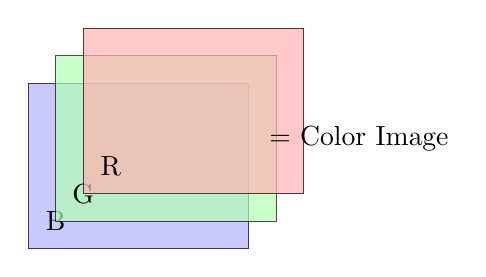
\begin{tikzpicture}[scale=0.7]
			\draw[fill=blue!30, opacity=0.7] (0,0) rectangle (4,3); \node at (0.5, 0.5) {B};
			\draw[fill=green!30, opacity=0.7] (0.5,0.5) rectangle (4.5,3.5); \node at (1, 1) {G};
			\draw[fill=red!30, opacity=0.7] (1,1) rectangle (5,4); \node at (1.5, 1.5) {R};
			\node at (6, 2) {= Color Image};
		\end{tikzpicture}
	\end{center}
	\textbf{OpenCV 的特殊性:} 默认读取顺序是 \highlight{BGR},而非 RGB。
\end{frame}

\begin{frame}[fragile]{互动练习:调色盘}
	如果一个像素的 RGB 值为以下数值,它是什么颜色?
	\begin{table}
		\centering
		\begin{tabular}{cccc}
			\toprule
			R   & G   & B   & 预测颜色                                  \\
			\midrule
			255 & 255 & 0   & \uncover<2->{\textcolor{yellow}{黄色}}  \\
			0   & 255 & 255 & \uncover<3->{\textcolor{cyan}{青色/浅蓝}} \\
			128 & 128 & 128 & \uncover<4->{\textcolor{gray}{灰色}}    \\
			0   & 0   & 0   & \uncover<5->{\textbf{黑色}}             \\
			\bottomrule
		\end{tabular}
	\end{table}
\end{frame}

\begin{frame}[fragile]{像素级操作:NumPy数组操作}
	\begin{columns}
		\column{0.5\textwidth}
		\textbf{基础索引与切片:}
		\begin{lstlisting}[language=Python, basicstyle=\ttfamily\tiny]
# 获取单个像素
pixel = img[100, 200]  # 返回[B, G, R]

# 获取红色通道
red_channel = img[:, :, 2]

# 获取左上角100x100区域
top_left = img[0:100, 0:100]

# 水平翻转(左右颠倒)
flipped = img[:, ::-1, :]
		\end{lstlisting}

		\vspace{0.2cm}
		\textbf{条件操作:}
		\begin{lstlisting}[language=Python, basicstyle=\ttfamily\tiny]
# 找出所有暗像素(值 < 128)
dark_pixels = img < 128

# 将暗像素增强
img[dark_pixels] = img[dark_pixels] * 1.2
		\end{lstlisting}

		\column{0.5\textwidth}
		\textbf{统计操作:}
		\begin{lstlisting}[language=Python, basicstyle=\ttfamily\tiny]
# 计算平均值
mean_val = np.mean(img)

# 计算标准差
std_val = np.std(img)

# 找最大最小值
max_val = np.max(img)
min_val = np.min(img)

# 计算非零像素数量
nonzero_count = np.count_nonzero(img)
		\end{lstlisting}

		\vspace{0.2cm}
		\begin{alertblock}{重要提示}
		NumPy切片是\textbf{视图(view)}而非副本,修改切片会影响原图!
		如果需要独立副本,使用\texttt{img.copy()}
		\end{alertblock}
	\end{columns}
\end{frame}

\begin{frame}[fragile]{像素级操作:手动实现灰度化}
	\textbf{原理:} $Gray = R \times 0.299 + G \times 0.587 + B \times 0.114$

	\begin{columns}
		\column{0.5\textwidth}
		\textbf{方法1:手动循环(学习用,不推荐)}
		\begin{lstlisting}[language=Python, basicstyle=\ttfamily\tiny]
def manual_grayscale(img):
    """手动实现灰度化"""
    h, w, c = img.shape
    gray = np.zeros((h, w), dtype=np.uint8)

    for i in range(h):
        for j in range(w):
            b, g, r = img[i, j]
            gray[i, j] = int(0.299*r +
                             0.587*g +
                             0.114*b)
    return gray
		\end{lstlisting}
		\textit{缺点:速度慢,不推荐生产环境使用}

		\column{0.5\textwidth}
		\textbf{方法2:向量化操作(推荐)}
		\begin{lstlisting}[language=Python, basicstyle=\ttfamily\tiny]
def grayscale_vectorized(img):
    """向量化实现灰度化"""
    # 方法1:矩阵运算
    b, g, r = cv2.split(img)
    gray = 0.299*r + 0.587*g + 0.114*b
    return gray.astype(np.uint8)

    # 方法2:点积(更简洁)
    weights = np.array([0.114, 0.587, 0.299])
    gray = img.dot(weights).astype(np.uint8)
    return gray
		\end{lstlisting}
		\textit{优点:速度快,利用NumPy向量化加速}
	\end{columns}

	\vspace{0.3cm}
	\begin{center}
		\textbf{性能对比:} 手动循环 \texttt{200ms} vs 向量化操作 \texttt{5ms}(快40倍)
	\end{center}
\end{frame}

\begin{frame}[fragile]{像素级操作:亮度调整的"溢出"陷阱}
	\begin{columns}
		\column{0.5\textwidth}
		\textbf{❌ 错误做法:}
		\begin{lstlisting}[language=Python, basicstyle=\ttfamily\tiny]
img = cv2.imread('exam.jpg')

# 直接相加
bright = img + 50

# 问题:如果像素值是220,
# 220 + 50 = 270
# 但uint8的范围是0-255
# 270会截断为14(或绕回)
# 导致图像出现噪点!
		\end{lstlisting}

		\vspace{0.2cm}
		\begin{alertblock}{为什么?}
		uint8类型:8位无符号整数\\
		范围:$[0, 255]$\\
		溢出:截断到边界值
		\end{alertblock}

		\column{0.5\textwidth}
		\textbf{✅ 正确做法:}
		\begin{lstlisting}[language=Python, basicstyle=\ttfamily\tiny]
# 方法1:使用np.clip
bright = np.clip(
    img.astype(np.int32) + 50,
    0, 255
).astype(np.uint8)

# 方法2:使用cv2.add(推荐)
bright = cv2.add(
    img,
    np.array([50.0])
)

# 方法3:使用convertScaleAbs
bright = cv2.convertScaleAbs(
    img,
    alpha=1.0,  # 对比度
    beta=50     # 亮度增量
)
		\end{lstlisting}
	\end{columns}

	\vspace{0.3cm}
	\begin{block}{核心原理}
		先转为int32类型(支持大范围),再clip到[0, 255],最后转回uint8
	\end{block}
\end{frame}

% 直方图理论
\begin{frame}[fragile]{图像的统计特性:直方图 (Histogram)}
	\begin{columns}
		\column{0.5\textwidth}
		\textbf{什么是直方图?}
		\begin{itemize}
			\item 横坐标:亮度级别 (0-255)
			\item 纵坐标:该亮度像素出现的频次
		\end{itemize}

		\textbf{在阅卷中的意义:}
		\begin{itemize}
			\item \highlight{曝光检查}:判断照片是否太暗或过曝
			\item \highlight{二值化参考}:寻找波谷作为分割阈值
		\end{itemize}

		\column{0.5\textwidth}
		\begin{lstlisting}[language=Python, basicstyle=\ttfamily\tiny]
import cv2
import matplotlib.pyplot as plt

# 计算直方图
img = cv2.imread('exam.jpg',
                 cv2.IMREAD_GRAYSCALE)
hist = cv2.calcHist([img], [0], None,
                    [256], [0, 256])

plt.plot(hist)
plt.title('Pixel Intensity Distribution')
plt.show()
		\end{lstlisting}

		\begin{center}
			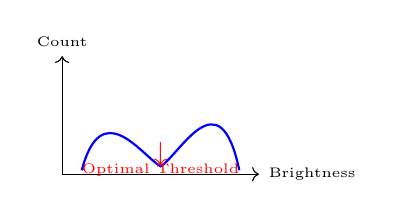
\begin{tikzpicture}[scale=0.5]
				\draw[->] (0,0) -- (5,0) node[right] {\tiny Brightness};
				\draw[->] (0,0) -- (0,3) node[above] {\tiny Count};
				\draw[thick, blue] (0.5,0.1) .. controls (1,2) and (2,0.5) .. (2.5,0.2) .. controls (3,0.5) and (4,2.5) .. (4.5,0.1);
				\node[red] at (2.5, 0.5) {$\downarrow$};
				\node[red, below] at (2.5, 0.5) {\tiny Optimal Threshold};
			\end{tikzpicture}
		\end{center}
	\end{columns}
\end{frame}

\begin{frame}[fragile]{直方图形态分析:试卷照片的曝光诊断}
	\textbf{场景:}自动判断试卷照片的质量

	\begin{columns}
		\column{0.5\textwidth}
		\textbf{1. 正常曝光(双峰分布)}
		\begin{itemize}
			\item 白纸(高亮度)+ 黑字(低亮度)
			\item 波谷在中间,适合二值化
			\item \textcolor{green!60!black}{\textbf{阅卷理想状态}}
		\end{itemize}

		\textbf{2. 欠曝(左偏分布)}
		\begin{itemize}
			\item 大部分像素集中在暗部
			\item 可能是光照不足
			\item 需要亮度增强
		\end{itemize}

		\textbf{3. 过曝(右偏分布)}
		\begin{itemize}
			\item 大部分像素集中在亮部
			\item 可能是闪光灯太强
			\item 需要降低亮度
		\end{itemize}

		\column{0.5\textwidth}
		\begin{lstlisting}[language=Python, basicstyle=\ttfamily\tiny]
def check_exposure(img):
    """检查图像曝光情况"""
    gray = cv2.cvtColor(img,
                       cv2.COLOR_BGR2GRAY)

    # 计算平均亮度
    mean_brightness = np.mean(gray)

    # 判断曝光状态
    if mean_brightness < 80:
        return "欠曝,建议增强"
    elif mean_brightness > 200:
        return "过曝,建议降低"
    else:
        return "曝光正常"

# 使用
status = check_exposure(img)
print(f"曝光状态: {status}")
		\end{lstlisting}
	\end{columns}
\end{frame}

\begin{frame}[fragile]{图像缩放:插值算法对比}
	\textbf{问题:}cv2.resize 时,像素是如何"凭空产生"或"消失"的?

	\begin{columns}
		\column{0.5\textwidth}
		\begin{lstlisting}[language=Python, basicstyle=\ttfamily\tiny]
import cv2
import numpy as np

img = cv2.imread('exam.jpg')
h, w = img.shape[:2]

# 1. 最近邻插值(最快)
# 取最近的像素值,会有马赛克
near = cv2.resize(img, (w*2, h*2),
                  interpolation=cv2.INTER_NEAREST)

# 2. 双线性插值(默认)
# 周围4个像素加权平均,较平滑
linear = cv2.resize(img, (w*2, h*2),
                   interpolation=cv2.INTER_LINEAR)

# 3. 双三次插值(最慢但最好)
# 周围16个像素加权平均
cubic = cv2.resize(img, (w*2, h*2),
                  interpolation=cv2.INTER_CUBIC)
		\end{lstlisting}

		\column{0.5\textwidth}
		\textbf{插值效果对比:}
		\begin{itemize}
			\item \textbf{最近邻}:
			      \begin{itemize}
				      \item 速度:最快
				      \item 质量:有锯齿
				      \item 应用:像素风游戏
			      \end{itemize}
			\item \textbf{双线性}:
			      \begin{itemize}
				      \item 速度:中等
				      \item 质量:较平滑
				      \item 应用:日常缩放
			      \end{itemize}
			\item \textbf{双三次}:
			      \begin{itemize}
				      \item 速度:最慢
				      \item 质量:最平滑
				      \item 应用:高质量缩放
			      \end{itemize}
		\end{itemize}

		\vspace{0.2cm}
		\textbf{阅卷建议:}
		\begin{itemize}
			\item 缩小用 \texttt{INTER\_AREA}(抗锯齿)
			\item 放大用 \texttt{INTER\_CUBIC}(高质量)
		\end{itemize}
	\end{columns}
\end{frame}

%=============================================================================
% 模块三:OpenCV 基础与进阶操作
%=============================================================================

\section{OpenCV 基础}

\begin{frame}[fragile]{OpenCV 核心函数详解}
	\begin{lstlisting}[title={图像读取的隐患}]
import cv2

# 路径千万不能有中文(新手常见错误)
img = cv2.imread('paper.jpg')

# 检查是否读取成功
if img is None:
    print("错误:文件不存在或路径含有中文!")

# 打印维度 (H, W, C)
print(img.shape)
	\end{lstlisting}

	\begin{block}{常用 Flag}
		\begin{itemize}
			\item \texttt{cv2.IMREAD\_COLOR}:加载彩色图(默认)
			\item \texttt{cv2.IMREAD\_GRAYSCALE}:直接以灰度模式加载
		\end{itemize}
	\end{block}
\end{frame}

\begin{frame}[fragile]{工程实战:处理中文路径的"终极方案"}
	\begin{alertblock}{真实场景}
		阅卷系统中,学生姓名经常是中文,文件名如:\texttt{张三\_试卷.jpg}\\
		\texttt{cv2.imread()} 直接读取会失败(返回 None)
	\end{alertblock}

	\begin{columns}
		\column{0.5\textwidth}
		\textbf{问题原因:}
		\begin{itemize}
			\item OpenCV 的 C++ 库不支持 Unicode 路径
			\item 中文路径会乱码
		\end{itemize}

		\vspace{0.3cm}
		\textbf{错误做法:}
		\begin{lstlisting}[language=Python, basicstyle=\ttfamily\tiny]
# 直接读取,返回 None
img = cv2.imread('张三_试卷.jpg')
if img is None:
    print("读取失败!")
		\end{lstlisting}

		\column{0.5\textwidth}
		\textbf{正确做法:}
		\begin{lstlisting}[language=Python, basicstyle=\ttfamily\tiny]
import cv2
import numpy as np

def imread_chinese(path):
    """读取中文路径的图片"""
    img_array = np.fromfile(path, 
                            dtype=np.uint8)
    img = cv2.imdecode(img_array, -1)
    return img

# 使用
img = imread_chinese('张三_试卷.jpg')
cv2.imshow('成功!', img)
		\end{lstlisting}
	\end{columns}
\end{frame}

\begin{frame}[fragile]{工程实战:保存中文路径图片}
	\textbf{配套技巧:}保存时也支持中文路径

	\begin{columns}
		\column{0.5\textwidth}
		\begin{lstlisting}[language=Python, basicstyle=\ttfamily\tiny]
import cv2
import numpy as np

def imwrite_chinese(path, img):
    """保存中文路径的图片"""
    is_success, img_buf = cv2.imencode(
        ".jpg", img)
    if is_success:
        img_buf.tofile(path)
        return True
    return False

# 使用
img = cv2.imread('exam.jpg')
imwrite_chinese('处理结果_张三.jpg', img)
print("保存成功!")
		\end{lstlisting}

		\column{0.5\textwidth}
		\textbf{原理说明:}
		\begin{enumerate}
			\item \textbf{imdecode}:从内存中的字节数组解码
			\item \textbf{imencode + tofile}:编码为字节数组后写入
		\end{enumerate}

		\vspace{0.3cm}
		\textbf{阅卷系统应用:}
		\begin{itemize}
			\item 批量处理学生试卷
			\item 生成带学生姓名的结果文件
		\end{itemize}
	\end{columns}
\end{frame}

\begin{frame}[fragile]{Matplotlib 显示与 BGR 转换}
	为什么用 \texttt{plt.imshow} 显示出来的人脸是青蓝色的?

	\begin{lstlisting}[language=Python, basicstyle=\ttfamily\small]
import matplotlib.pyplot as plt

# OpenCV 是 BGR,Matplotlib 是 RGB
img_rgb = cv2.cvtColor(img, cv2.COLOR_BGR2RGB)

plt.imshow(img_rgb)
plt.show()
	\end{lstlisting}

	\vspace{0.3cm}
	\textbf{注意:} 灰度图显示时需要设置 \texttt{cmap='gray'},否则会变成"原油色"。

	\begin{lstlisting}[language=Python, basicstyle=\ttfamily\small]
plt.imshow(gray_img, cmap='gray')
	\end{lstlisting}
\end{frame}

\begin{frame}[fragile]{OpenCV进阶:几何变换}
	\begin{columns}
		\column{0.5\textwidth}
		\textbf{1. 平移(Translation)}
		\begin{lstlisting}[language=Python, basicstyle=\ttfamily\tiny]
# 向右平移100,向下平移50
M = np.float32([
    [1, 0, 100],  # x位移
    [0, 1, 50]   # y位移
])
translated = cv2.warpAffine(
    img, M, (w, h)
)
		\end{lstlisting}

		\vspace{0.2cm}
		\textbf{2. 旋转(Rotation)}
		\begin{lstlisting}[language=Python, basicstyle=\ttfamily\tiny]
# 逆时针旋转30度
center = (w//2, h//2)  # 旋转中心
M = cv2.getRotationMatrix2D(
    center,
    30,     # 角度(度)
    1.0     # 缩放比例
)
rotated = cv2.warpAffine(
    img, M, (w, h)
)
		\end{lstlisting}

		\column{0.5\textwidth}
		\textbf{3. 缩放(Scaling)}
		\begin{lstlisting}[language=Python, basicstyle=\ttfamily\tiny]
# 放大2倍
scaled = cv2.resize(
    img,
    None,
    fx=2.0,
    fy=2.0,
    interpolation=cv2.INTER_CUBIC
)

# 指定尺寸缩放
resized = cv2.resize(
    img,
    (800, 600),  # 宽, 高
    interpolation=cv2.INTER_LINEAR
)
		\end{lstlisting}

		\vspace{0.2cm}
		\begin{block}{插值方法选择}
		\begin{itemize}
			\item 放大:\texttt{INTER\_CUBIC}(质量最好)
			\item 缩小:\texttt{INTER\_AREA}(抗锯齿)
			\item 快速:\texttt{INTER\_LINEAR}
		\end{itemize}
		\end{block}
	\end{columns}
\end{frame}

\begin{frame}[fragile]{OpenCV进阶:仿射变换与透视变换}
	\begin{columns}
		\column{0.5\textwidth}
		\textbf{仿射变换(Affine Transform)}
		\begin{itemize}
			\item 保持平行线的平行性
			\item 需要3个点对应
		\end{itemize}
		\begin{lstlisting}[language=Python, basicstyle=\ttfamily\tiny]
# 原图像的3个点
src_pts = np.float32([
    [50, 50],    # 左上
    [200, 50],   # 右上
    [50, 200]    # 左下
])

# 目标图像的3个点
dst_pts = np.float32([
    [10, 10],
    [200, 20],
    [10, 200]
])

# 计算变换矩阵
M = cv2.getAffineTransform(
    src_pts, dst_pts
)

# 执行变换
affine = cv2.warpAffine(
    img, M, (w, h)
)
		\end{lstlisting}

		\column{0.5\textwidth}
		\textbf{透视变换(Perspective Transform)}
		\begin{itemize}
			\item 不保持平行性
			\item 需要4个点对应
			\item \highlight{下周重点!}
		\end{itemize}
		\begin{lstlisting}[language=Python, basicstyle=\ttfamily\tiny]
# 原图像的4个角点
src_pts = np.float32([
    [100, 150],  # 左上
    [450, 120],  # 右上
    [480, 380],  # 右下
    [80, 400]    # 左下
])

# 目标矩形
width, height = 400, 300
dst_pts = np.float32([
    [0, 0],
    [width-1, 0],
    [width-1, height-1],
    [0, height-1]
])

# 计算变换矩阵
M = cv2.getPerspectiveTransform(
    src_pts, dst_pts
)

# 执行变换
warped = cv2.warpPerspective(
    img, M, (width, height)
)
		\end{lstlisting}
	\end{columns}
\end{frame}

\begin{frame}[fragile]{OpenCV进阶:形态学操作基础}
	\textbf{形态学操作:} 基于图像形状的变换,常用于二值图像

	\begin{columns}
		\column{0.5\textwidth}
		\textbf{1. 腐蚀(Erosion)}
		\begin{itemize}
			\item 膨胀白色,收缩黑色
			\item 去除小噪点
		\end{itemize}
		\begin{lstlisting}[language=Python, basicstyle=\ttfamily\tiny]
kernel = np.ones((3, 3), np.uint8)
eroded = cv2.erode(binary, kernel, 
                   iterations=1)
		\end{lstlisting}

		\vspace{0.2cm}
		\textbf{2. 膨胀(Dilation)}
		\begin{itemize}
			\item 收缩白色,膨胀黑色
			\item 填充小孔洞
		\end{itemize}
		\begin{lstlisting}[language=Python, basicstyle=\ttfamily\tiny]
dilated = cv2.dilate(binary, kernel, 
                     iterations=1)
		\end{lstlisting}

		\vspace{0.2cm}
		\textbf{3. 开运算(Opening)}
		\begin{itemize}
			\item 先腐蚀后膨胀
			\item 去除小物体,保持大物体
		\end{itemize}
		\begin{lstlisting}[language=Python, basicstyle=\ttfamily\tiny]
opening = cv2.morphologyEx(
    binary, cv2.MORPH_OPEN, kernel
)
		\end{lstlisting}

		\column{0.5\textwidth}
		\textbf{4. 闭运算(Closing)}
		\begin{itemize}
			\item 先膨胀后腐蚀
			\item 填充小孔洞,连接近邻物体
		\end{itemize}
		\begin{lstlisting}[language=Python, basicstyle=\ttfamily\tiny]
closing = cv2.morphologyEx(
    binary, cv2.MORPH_CLOSE, kernel
)
		\end{lstlisting}

		\vspace{0.2cm}
		\textbf{5. 形态学梯度}
		\begin{itemize}
			\item 膨胀 - 腐蚀
			\item 提取边缘
		\end{itemize}
		\begin{lstlisting}[language=Python, basicstyle=\ttfamily\tiny]
gradient = cv2.morphologyEx(
    binary, cv2.MORPH_GRADIENT, 
    kernel
)
		\end{lstlisting}

		\vspace{0.2cm}
		\begin{block}{结构元素(Kernel)}
		可自定义形状:矩形、十字形、椭圆形\\
		大小决定影响范围
		\end{block}
	\end{columns}
\end{frame}

\begin{frame}[fragile]{形态学操作在阅卷中的应用}
	\begin{columns}
		\column{0.5\textwidth}
		\textbf{场景1:去除填涂噪点}
		\begin{itemize}
			\item 问题:填涂边缘有细小噪点
			\item 解决:开运算去除小噪点
		\end{itemize}
		\begin{lstlisting}[language=Python, basicstyle=\ttfamily\tiny]
# 去除小噪点
kernel = np.ones((2, 2), np.uint8)
clean_bubble = cv2.morphologyEx(
    binary,
    cv2.MORPH_OPEN,
    kernel
)
		\end{lstlisting}

		\vspace{0.2cm}
		\textbf{场景2:连接断开的笔迹}
		\begin{itemize}
			\item 问题:手写数字断开
			\item 解决:闭运算连接
		\end{itemize}
		\begin{lstlisting}[language=Python, basicstyle=\ttfamily\tiny]
# 连接断开部分
kernel = np.ones((3, 3), np.uint8)
connected = cv2.morphologyEx(
    binary,
    cv2.MORPH_CLOSE,
    kernel
)
		\end{lstlisting}

		\column{0.5\textwidth}
		\textbf{场景3:提取轮廓边缘}
		\begin{itemize}
			\item 问题:需要清晰的轮廓
			\item 解决:形态学梯度
		\end{itemize}
		\begin{lstlisting}[language=Python, basicstyle=\ttfamily\tiny]
# 提取边缘
gradient = cv2.morphologyEx(
    binary,
    cv2.MORPH_GRADIENT,
    kernel
)
		\end{lstlisting}

		\vspace{0.2cm}
		\begin{block}{可视化对比}
		\begin{itemize}
			\item 原始:有噪点的填涂
			\item 开运算:干净的填涂
			\item 闭运算:连接的笔迹
			\item 梯度:清晰的边缘
		\end{itemize}
		\end{block}

		\vspace{0.2cm}
		\begin{center}
			\highlight{形态学操作是图像预处理的"外科手术刀"}
		\end{center}
	\end{columns}
\end{frame}

%=============================================================================
% 模块四:核心算法与实战演练
%=============================================================================

\section{图像滤镜原理}

\begin{frame}[fragile]{滤镜 1:灰度化 (Grayscale)}
	\textbf{为什么要灰度化?}
	\begin{itemize}
		\item 减少计算量(数据量降至 1/3)
		\item 识别试卷上的文字,颜色信息通常是不必要的
	\end{itemize}
	\textbf{原理:} $Gray = R \times 0.299 + G \times 0.587 + B \times 0.114$
	\\ (为什么绿色权重最高?因为人眼对绿色最敏感。)

	\begin{lstlisting}[language=Python, basicstyle=\ttfamily\small]
# 方法1:OpenCV 函数
gray = cv2.cvtColor(img, cv2.COLOR_BGR2GRAY)

# 方法2:手动计算(不推荐)
gray = 0.299 * r + 0.587 * g + 0.114 * b
\end{lstlisting}
\end{frame}

\begin{frame}[fragile]{滤镜 2:反色 (Inversion)}
	\textbf{原理:} $NewValue = 255 - OldValue$
	\begin{itemize}
		\item 黑色 (0) $\to$ 白色 (255)
		\item 白色 (255) $\to$ 黑色 (0)
	\end{itemize}
	\textbf{应用:} 增强暗背景下的试卷特征,或者扫描负片。

	\begin{lstlisting}[language=Python, basicstyle=\ttfamily\small]
# 方法1:NumPy 运算
inverted = 255 - img

# 方法2:OpenCV 位运算
inverted = cv2.bitwise_not(img)

# 方法3:NumPy 按位取反
inverted = np.bitwise_not(img)
\end{lstlisting}
\end{frame}

\begin{frame}[fragile]{滤镜 3:亮度调整与"溢出"陷阱}
	\textbf{错误做法:} \texttt{img + 50}
	\\ 如果像素值是 220,加 50 变成 270。而在 \texttt{uint8} 类型下,270 会变成 \highlight{14} (截断/绕回),导致图像出现难看的噪点。

	\begin{lstlisting}[title={安全写法}]
# 使用 numpy 的 clip 函数限制范围
bright_img = np.clip(img.astype(np.int32) + 50, 0, 255).astype(np.uint8)

# 或者使用 OpenCV 内置函数(推荐,速度更快)
bright_img = cv2.add(img, np.array([50.0]))
\end{lstlisting}
\end{frame}

% -----------------------------------------------------------------------------
% 代码实战环节
% -----------------------------------------------------------------------------

\section{代码实战}

\begin{frame}[fragile]{代码实战(1/5):图像翻转与旋转}
	\textbf{场景:}阅卷时试卷可能被倒置,需要自动旋转

	\begin{columns}
		\column{0.5\textwidth}
		\begin{lstlisting}[language=Python, basicstyle=\ttfamily\tiny]
import cv2
import numpy as np

img = cv2.imread('exam.jpg')

# 方法1:NumPy 数组切片
# 垂直翻转(上下颠倒)
flip_v = img[::-1, :, :]

# 水平翻转(左右颠倒)
flip_h = img[:, ::-1, :]

# 水平+垂直翻转(旋转180度)
flip_both = img[::-1, ::-1, :]
\end{lstlisting}

		\column{0.5\textwidth}
		\begin{lstlisting}[language=Python, basicstyle=\ttfamily\tiny]
# 方法2:OpenCV 函数(推荐)
flip_v = cv2.flip(img, 0)      # 垂直
flip_h = cv2.flip(img, 1)      # 水平
flip_both = cv2.flip(img, -1)  # 两者

# 显示对比
cv2.imshow('Original', img)
cv2.imshow('Flip V', flip_v)
cv2.imshow('Flip H', flip_h)
cv2.waitKey(0)
\end{lstlisting}
	\end{columns}

	\vspace{0.2cm}
	\textbf{性能对比:} NumPy 切片比 cv2.flip 快约 20\%,但 cv2.flip 更易读
\end{frame}

\begin{frame}[fragile]{代码实战(2/5):提取答题卡区域(ROI)}
	\textbf{场景:}从整张试卷中提取答题卡区域

	\begin{columns}
		\column{0.5\textwidth}
		\begin{lstlisting}[language=Python, basicstyle=\ttfamily\tiny]
import cv2
import numpy as np

exam = cv2.imread('exam.jpg')
h, w = exam.shape[:2]

# 假设答题卡在右下角
# 坐标:从宽度的60%到末尾,高度的50%到末尾
x1, x2 = int(w * 0.6), w
y1, y2 = int(h * 0.5), h

# 提取 ROI
roi = exam[y1:y2, x1:x2]

# 保存 ROI
cv2.imwrite('answer_sheet.jpg', roi)

print("原图大小:", exam.shape)
print("ROI 大小:", roi.shape)
\end{lstlisting}

		\column{0.5\textwidth}
		\textbf{坐标系统回顾:}
		\begin{itemize}
			\item 原点在左上角 (0, 0)
			\item \texttt{img[y1:y2, x1:x2]}
			\item y 是行(高度),x 是列(宽度)
		\end{itemize}

		\vspace{0.3cm}
		\begin{center}
			\begin{tikzpicture}[scale=0.4]
				\draw[thick, fill=blue!10] (0,0) rectangle (6,4);
				\node at (3,2) {整张试卷};
				\draw[thick, fill=red!30] (3.5,0) rectangle (6,2);
				\node at (4.75,1) {\tiny ROI};
				\draw[->] (3.5,2) -- (3.5,3) node[above] {\tiny y1};
				\draw[->] (3.5,0) -- (3.5,-1) node[below] {\tiny y2};
				\draw[->] (3.5,1) -- (2.5,1) node[left] {\tiny x1};
				\draw[->] (6,1) -- (7,1) node[right] {\tiny x2};
			\end{tikzpicture}
		\end{center}
	\end{columns}
\end{frame}

\begin{frame}[fragile]{代码实战(3/5):通道分离与合并}
	\textbf{场景:}提取特定颜色通道

	\begin{columns}
		\column{0.5\textwidth}
		\begin{lstlisting}[language=Python, basicstyle=\ttfamily\tiny]
import cv2

img = cv2.imread('exam.jpg')

# 方法1:使用 split 函数
b, g, r = cv2.split(img)

# 只保留红色通道,其他设为0
zeros = np.zeros_like(b)
img_r = cv2.merge([zeros, zeros, r])
\end{lstlisting}

		\vspace{0.2cm}
		\begin{lstlisting}[language=Python, basicstyle=\ttfamily\tiny]
# 方法2:直接索引(更快)
img_r = img.copy()
img_r[:, :, 0] = 0  # B通道
img_r[:, :, 1] = 0  # G通道
# R通道保持不变

cv2.imshow('Red Only', img_r)
cv2.waitKey(0)
\end{lstlisting}

		\column{0.5\textwidth}
		\textbf{通道顺序:}
		\begin{itemize}
			\item OpenCV: \textbf{BGR}
			\item matplotlib: \textbf{RGB}
			\item PIL: \textbf{RGB}
		\end{itemize}

		\vspace{0.3cm}
		\begin{alertblock}{常见错误}
			使用 \texttt{plt.imshow(img)} 显示 OpenCV 图像时,颜色会异常!
		\end{alertblock}

		\vspace{0.2cm}
		\textbf{解决方案:}
		\begin{lstlisting}[language=Python, basicstyle=\ttfamily\tiny]
img_rgb = cv2.cvtColor(img, cv2.COLOR_BGR2RGB)
plt.imshow(img_rgb)
\end{lstlisting}
	\end{columns}
\end{frame}

\begin{frame}[fragile]{代码实战(4/5):阅卷系统核心代码}
	\textbf{场景:}检测答题卡填涂位置

	\begin{columns}
		\column{0.5\textwidth}
		\begin{lstlisting}[language=Python, basicstyle=\ttfamily\tiny]
import cv2
import numpy as np

# 1. 读取答题卡区域
roi = cv2.imread('answer_sheet.jpg',
                 cv2.IMREAD_GRAYSCALE)

# 2. 二值化
_, binary = cv2.threshold(roi, 127, 255,
                          cv2.THRESH_BINARY)

# 3. 定义选项位置
positions = [
    (100, 100, 120, 120),  # A
    (100, 130, 120, 150),  # B
    (100, 160, 120, 180),  # C
    (100, 190, 120, 200)   # D
]
\end{lstlisting}

		\column{0.5\textwidth}
		\begin{lstlisting}[language=Python, basicstyle=\ttfamily\tiny]
# 4. 检测每个选项是否被填涂
answers = []
for (x1, y1, x2, y2) in positions:
    option = binary[y1:y2, x1:x2]

    # 计算黑色像素比例
    black_pixels = np.sum(option == 0)
    total_pixels = option.size
    ratio = black_pixels / total_pixels

    # 判断是否填涂(阈值30%)
    if ratio > 0.3:
        answers.append('填涂')
    else:
        answers.append('未填')

print(answers)
\end{lstlisting}
	\end{columns}

	\vspace{0.2cm}
	\textbf{核心思想:}填涂区域黑色像素占比显著高于未填涂区域
\end{frame}

\begin{frame}[fragile]{代码实战(5/5):图像增强对比}
	\textbf{场景:}答题卡光照不均,需要增强对比度

	\begin{columns}
		\column{0.5\textwidth}
		\begin{lstlisting}[language=Python, basicstyle=\ttfamily\tiny]
import cv2
import numpy as np

img = cv2.imread('exam.jpg')

# 方法1:线性对比度调整
# new = alpha * old + beta
enhanced = cv2.convertScaleAbs(
    img, alpha=1.5, beta=30
)
\end{lstlisting}

		\vspace{0.2cm}
		\begin{lstlisting}[language=Python, basicstyle=\ttfamily\tiny]
# 方法2:直方图均衡化
gray = cv2.cvtColor(img, cv2.COLOR_BGR2GRAY)
equalized = cv2.equalizeHist(gray)
\end{lstlisting}

		\column{0.5\textwidth}
		\begin{lstlisting}[language=Python, basicstyle=\ttfamily\tiny]
# 方法3:CLAHE(自适应)
clahe = cv2.createCLAHE(
    clipLimit=2.0,
    tileGridSize=(8,8)
)
enhanced_clahe = clahe.apply(gray)
\end{lstlisting}

		\vspace{0.2cm}
		\textbf{效果对比:}
		\begin{itemize}
			\item \textbf{线性调整}:简单但效果有限
			\item \textbf{直方图均衡化}:全局优化
			\item \textbf{CLAHE}:局部自适应,效果最好
		\end{itemize}

		\vspace{0.2cm}
		\textbf{阅卷推荐:} CLAHE 适合光照不均场景
	\end{columns}
\end{frame}

% -----------------------------------------------------------------------------
% 完整阅卷系统Live Coding
% -----------------------------------------------------------------------------

\begin{frame}[fragile]{Live Coding:完整的阅卷预处理流程}
	\textbf{目标:} 从照片到可识别的图像

	\begin{columns}
		\column{0.5\textwidth}
		\begin{lstlisting}[language=Python, basicstyle=\ttfamily\tiny]
def preprocess_exam(image_path):
    """试卷预处理完整流程"""

    # 1. 读取图像(支持中文路径)
    img = imread_chinese(image_path)

    # 2. 转为灰度
    gray = cv2.cvtColor(img,
                       cv2.COLOR_BGR2GRAY)

    # 3. 去噪
    denoised = cv2.GaussianBlur(
        gray, (5, 5), 0)

    # 4. 对比度增强(CLAHE)
    clahe = cv2.createCLAHE(2.0, (8, 8))
    enhanced = clahe.apply(denoised)

    # 5. 二值化
    binary = cv2.adaptiveThreshold(
        enhanced, 255,
        cv2.ADAPTIVE_THRESH_GAUSSIAN_C,
        cv2.THRESH_BINARY, 11, 2)

    return img, gray, enhanced, binary

# 使用
img, gray, enhanced, binary = \
    preprocess_exam('exam.jpg')
		\end{lstlisting}

		\column{0.5\textwidth}
		\textbf{流程图:}
		\begin{center}
			\begin{tikzpicture}[scale=0.6, node distance=0.8cm]
				\node[draw, rounded corners] (1) {原图};
				\node[draw, rounded corners, below of=1] (2) {灰度};
				\node[draw, rounded corners, below of=2] (3) {去噪};
				\node[draw, rounded corners, below of=3] (4) {增强};
				\node[draw, rounded corners, below of=4] (5) {二值};

				\draw[->] (1) -- (2);
				\draw[->] (2) -- (3);
				\draw[->] (3) -- (4);
				\draw[->] (4) -- (5);
			\end{tikzpicture}
		\end{center}

		\vspace{0.2cm}
		\textbf{展示结果:}
		\begin{itemize}
			\item 原始照片
			\item 预处理后图像
			\item 处理时间对比
		\end{itemize}
	\end{columns}
\end{frame}

\begin{frame}[fragile]{Live Coding:阅卷系统核心检测}
	\textbf{功能1:填涂检测}
	\begin{lstlisting}[language=Python, basicstyle=\ttfamily\tiny]
def detect_bubble(binary, position):
    """检测单个气泡的填涂状态"""
    x1, y1, x2, y2 = position

    # 提取气泡区域
    bubble = binary[y1:y2, x1:x2]

    # 计算填涂密度
    black_pixels = np.sum(bubble == 0)
    total_pixels = bubble.size
    fill_ratio = black_pixels / total_pixels

    # 判断状态
    if fill_ratio > 0.6:
        return 'filled'
    elif fill_ratio < 0.2:
        return 'empty'
    else:
        return 'uncertain'
	\end{lstlisting}

	\vspace{0.2cm}
	\textbf{功能2:多选检测与警告}
	\begin{lstlisting}[language=Python, basicstyle=\ttfamily\tiny]
def detect_multiple_choice(binary, positions):
    """检测多选并警告"""
    results = []
    for pos in positions:
        state = detect_bubble(binary, pos)
        results.append(state)

    # 统计填涂数量
    filled_count = sum(1 for r in results if r == 'filled')

    if filled_count > 1:
        print(f"警告:检测到多选({filled_count}个选项)")

    return results
	\end{lstlisting}
\end{frame}

\begin{frame}[fragile]{Live Coding:图像质量检测函数}
	\textbf{目标:} 自动判断试卷照片是否适合识别

	\begin{columns}
		\column{0.5\textwidth}
		\begin{lstlisting}[language=Python, basicstyle=\ttfamily\tiny]
def check_image_quality(img):
    """检测图像质量"""

    h, w = img.shape[:2]

    # 1. 分辨率检查
    if min(h, w) < 1000:
        return False, "分辨率过低"

    # 2. 曝光检查
    gray = cv2.cvtColor(img,
                       cv2.COLOR_BGR2GRAY)
    mean_brightness = np.mean(gray)

    if mean_brightness < 80:
        return False, "曝光不足"
    elif mean_brightness > 200:
        return False, "过曝"

    # 3. 清晰度检查
    laplacian_var = cv2.Laplacian(
        gray, cv2.CV_64F
    ).var()

    if laplacian_var < 100:
        return False, "图像模糊"

    return True, "质量合格"
		\end{lstlisting}

		\column{0.5\textwidth}
		\textbf{使用示例:}
		\begin{lstlisting}[language=Python, basicstyle=\ttfamily\tiny]
img = imread_chinese('exam.jpg')

is_good, msg = check_image_quality(img)

if is_good:
    print(f"图像质量:{msg}")
    # 继续处理
    result = process_image(img)
else:
    print(f"图像质量:{msg}")
    print("提示用户重新拍照")
		\end{lstlisting}

		\vspace{0.2cm}
		\textbf{质量标准:}
		\begin{itemize}
			\item 分辨率:≥1000px
			\item 曝光:80-200
			\item 清晰度:Laplacian方差 ≥100
		\end{itemize}
	\end{columns}
\end{frame}

\begin{frame}[fragile]{Live Coding:批量处理与结果输出}
	\textbf{批量处理函数:}
	\begin{lstlisting}[language=Python, basicstyle=\ttfamily\tiny]
import os
import json

def batch_process_exams(folder_path, output_path):
    """批量处理试卷"""
    results = []

    for filename in os.listdir(folder_path):
        if not filename.endswith(('.jpg', '.png')):
            continue

        input_path = os.path.join(folder_path, filename)

        # 1. 质量检查
        is_good, msg = check_image_quality(
            imread_chinese(input_path))
        if not is_good:
            print(f"X {filename}: {msg}")
            continue

        # 2. 预处理
        img, gray, enhanced, binary = \
            preprocess_exam(input_path)

        # 3. 检测答题
        answers = detect_all_answers(binary)

        # 4. 评分
        score, details = grade_answers(answers)

        # 5. 保存结果
        result = {
            'filename': filename,
            'score': score,
            'details': details,
            'quality': is_good
        }
        results.append(result)

        print(f"OK {filename}: {score}分")

    # 保存到JSON
    with open(output_path, 'w', encoding='utf-8') as f:
        json.dump(results, f, ensure_ascii=False, indent=2)

    return results
	\end{lstlisting}
\end{frame}

%=============================================================================
% 模块五:工业硬件知识
%=============================================================================

\section{硬件知识}

\begin{frame}[fragile]{硬件知识(1/3):卷帘快门 vs 全局快门}
	\textbf{快门:控制传感器曝光时间的机制}

	\begin{columns}
		\column{0.5\textwidth}
		\textbf{卷帘快门}
		\begin{itemize}
			\item 逐行曝光,像"扫描"一样
			\item 优点:便宜、功耗低
			\item 缺点:拍摄快速物体会变形
			\item \highlight{斜坡效应}
			      \begin{itemize}
				      \item 照片上下部分时间不同
				      \item 快速物体会倾斜
			      \end{itemize}
		\end{itemize}

		\vspace{0.3cm}
		\textbf{应用:}手机摄像头、普通相机

		\column{0.5\textwidth}
		\textbf{全局快门}
		\begin{itemize}
			\item 所有像素同时曝光
			\item 优点:无变形
			\item 缺点:昂贵、功耗高
			\item 工业相机标配
		\end{itemize}

		\vspace{0.3cm}
		\textbf{应用:}工业检测、高速摄影

		\vspace{0.3cm}
		\begin{center}
			\begin{tikzpicture}[scale=0.3]
				\node[draw, fill=blue!20] (rolling) at (0,0) {卷帘快门};
				\node[draw, fill=green!20] (global) at (5,0) {全局快门};
				\draw[->] (rolling) -- (3,-2) node[midway,right] {\tiny 倾斜};
				\draw[->] (global) -- (8,-2) node[midway,right] {\tiny 正常};
			\end{tikzpicture}
		\end{center}
	\end{columns}

	\vspace{0.3cm}
	\begin{block}{阅卷系统建议}
		如果试卷传输速度快,需使用全局快门相机,避免文字倾斜变形
	\end{block}
\end{frame}

\begin{frame}[fragile]{硬件知识(2/3):CMOS vs CCD 传感器}
	\textbf{图像传感器:将光信号转换为电信号的芯片}

	\begin{columns}
		\column{0.5\textwidth}
		\textbf{CMOS 传感器}
		\begin{itemize}
			\item 每个像素有独立的放大器
			\item 优点:
			      \begin{itemize}
				      \item 速度快(并行读出)
				      \item 功耗低
				      \item 成本低
				      \item 集成度高
			      \end{itemize}
			\item 缺点:
			      \begin{itemize}
				      \item 噪声较大
				      \item 填充因子低
			      \end{itemize}
		\end{itemize}

		\vspace{0.2cm}
		\textbf{应用:}手机、网络摄像头、消费级相机

		\column{0.5\textwidth}
		\textbf{CCD 传感器}
		\begin{itemize}
			\item 所有电荷通过一个放大器
			\item 优点:
			      \begin{itemize}
				      \item 图像质量高
				      \item 噪声低
				      \item 动态范围大
				      \item 一致性好
			      \end{itemize}
			\item 缺点:
			      \begin{itemize}
				      \item 速度慢(串行读出)
				      \item 功耗高
				      \item 成本高
			      \end{itemize}
		\end{itemize}

		\vspace{0.2cm}
		\textbf{应用:}天文摄影、科学成像、高端相机
	\end{columns}

	\vspace{0.3cm}
	\begin{block}{阅卷系统选择}
		高速扫描仪使用 CMOS(速度快),精密分析可考虑 CCD(质量高)
	\end{block}
\end{frame}

\begin{frame}[fragile]{硬件知识(3/3):图像传感器关键参数}
	\textbf{选择相机时需要关注的参数}

	\begin{columns}
		\column{0.5\textwidth}
		\textbf{1. 分辨率}
		\begin{itemize}
			\item 像素数量:1920×1080, 4K等
			\item \highlight{不是越高越好!}
			\item 阅卷:300dpi 扫描足够
		\end{itemize}

		\vspace{0.2cm}
		\textbf{2. 帧率}
		\begin{itemize}
			\item 每秒传输图像数
			\item 高速扫描:30-60 fps
		\end{itemize}

		\vspace{0.2cm}
		\textbf{3. 像素尺寸}
		\begin{itemize}
			\item 单个像素物理大小(μm)
			\item 越大 = 进光量越大 = 噪声越低
			\item 手机:1.4μm,单反:5-8μm
		\end{itemize}

		\column{0.5\textwidth}
		\textbf{4. 动态范围}
		\begin{itemize}
			\item 能同时捕捉的最亮和最暗细节
			\item 单位:dB 或 stops
			\item 高端:60-80 dB
			\item 普通:40-60 dB
		\end{itemize}

		\vspace{0.2cm}
		\textbf{5. 信噪比(SNR)}
		\begin{itemize}
			\item 信号与噪声的比值
			\item 越高越好
			\item >40dB 为优秀
		\end{itemize}

		\vspace{0.2cm}
		\textbf{6. ISO 感光度}
		\begin{itemize}
			\item 对光的敏感程度
			\item 高 ISO:噪点多
			\item 阅卷:低 ISO(100-400)
		\end{itemize}
	\end{columns}

	\vspace{0.3cm}
	\begin{block}{阅卷系统推荐配置}
		分辨率:≥5MP | 帧率:≥30 fps | 快门:全局快门 | 接口:GigE/USB3.0
	\end{block}
\end{frame}

\begin{frame}[fragile]{工业相机选型指南}
	\textbf{阅卷系统相机选型决策树}

	\begin{columns}
		\column{0.5\textwidth}
		\textbf{根据吞吐量选择:}
		\begin{itemize}
			\item \textbf{小型(<1000张/天)}:USB3.0相机
			\item \textbf{中型(1000-10000张/天)}:GigE相机
			\item \textbf{大型(>10000张/天)}:Camera Link高速相机
		\end{itemize}

		\vspace{0.3cm}
		\textbf{根据精度选择:}
		\begin{itemize}
			\item \textbf{普通阅卷}:300dpi ≈ 5MP
			\item \textbf{手写识别}:600dpi ≈ 10MP
			\item \textbf{图表分析}:1200dpi ≈ 20MP
		\end{itemize}

		\column{0.5\textwidth}
		\textbf{热门品牌对比:}
		\begin{table}
			\centering
			\small
			\begin{tabular}{lccc}
				\toprule
				品牌 & 价格 & 质量 & 支持 \\
				\midrule
				Basler & 中 & 高 & 好 \\
				IDS & 中 & 高 & 好 \\
				海康 & 低 & 中 & 中 \\
				大华 & 低 & 中 & 中 \\
				\bottomrule
			\end{tabular}
		\end{table}

		\vspace{0.2cm}
		\textbf{接口选择:}
		\begin{itemize}
			\item \textbf{USB3.0}:短距离(<3m),即插即用
			\item \textbf{GigE}:长距离(<100m),需交换机
			\item \textbf{Camera Link}:超高速,专用线缆
		\end{itemize}
	\end{columns}
\end{frame}

\begin{frame}[fragile]{阅卷系统硬件配置建议}
	\textbf{完整硬件方案示例}

	\begin{columns}
		\column{0.5\textwidth}
		\textbf{方案A:经济型(学校用)}
		\begin{itemize}
			\item 相机:USB3.0工业相机(5MP,30fps)
			\item 镜头:定焦镜头(8mm, f/2.8)
			\item 光源:LED环形光(可调亮度)
			\item 传输:USB3.0线缆(2米)
			\item 预算:约5000-8000元
		\end{itemize}

		\vspace{0.3cm}
		\textbf{方案B:专业型(考试中心)}
		\begin{itemize}
			\item 相机:GigE全局快门(10MP,60fps)
			\item 镜头:远心镜头(低畸变)
			\item 光源:条形光源阵列
			\item 传输:千兆以太网
			\item 预算:约20000-30000元
		\end{itemize}

		\column{0.5\textwidth}
		\textbf{关键配置要点:}
		\begin{enumerate}
			\item \textbf{全局快门}:避免文字倾斜
			\item \textbf{镜头畸变<1\%}:保证定位精度
			\item \textbf{均匀照明}:光照变化<10\%
			\item \textbf{固定焦距}:避免自动对焦抖动
			\item \textbf{稳定支架}:减少震动影响
		\end{enumerate}

		\vspace{0.3cm}
		\begin{alertblock}{避坑指南}
			\begin{itemize}
				\item 不要用手机摄像头(卷帘快门)
				\item 不要用网络摄像头(分辨率低)
				\item 不要用自动对焦镜头(会漂移)
			\end{itemize}
		\end{alertblock}
	\end{columns}
\end{frame}

%=============================================================================
% 模块六:互动测验与Live Coding
%=============================================================================

\section{互动测验}

\begin{frame}[fragile]{小测验时间(1):NumPy 综合测试}
	\begin{block}{问题}
		给定形状为 (100, 100, 3) 的彩色图像,如何提取中心 50×50 的红色通道值?
		\begin{enumerate}[(A)]
			\item \texttt{img[25:75, 25:75, 0]}
			\item \texttt{img[25:75, 25:75, 2]}
			\item \texttt{img[50:100, 50:100, 2]}
			\item \texttt{img[25:75, 25:75]}
		\end{enumerate}
	\end{block}
	\pause
	\textbf{答案:} \highlight{B. img[25:75, 25:75, 2]} \\
	\vspace{0.2cm}
	\textbf{解析:}
	\begin{itemize}
		\item 100×100 图像的中心 50×50:索引从 25 到 75
		\item OpenCV 中 BGR 顺序,红色通道索引为 2
		\item \texttt{img[y1:y2, x1:x2, channel]} 格式
	\end{itemize}
\end{frame}

% -----------------------------------------------------------------------------
% Live Coding 闪电编程任务
% -----------------------------------------------------------------------------

\begin{frame}[fragile]{Live Coding(1/3):5分钟闪电编程任务}
	\begin{alertblock}{编程挑战}
		给定一张"脏"试卷图像(含噪声、光照不均)\\
		\textbf{任务:}在 5 分钟内,用 \highlight{3 行代码} 提取出学号区的均值
	\end{alertblock}

	\begin{columns}
		\column{0.5\textwidth}
		\textbf{提示:}
		\begin{enumerate}
			\item 读取图像(已有)
			\item 切片学号区
			\item 计算均值
		\end{enumerate}

		\vspace{0.3cm}
		\textbf{学号区位置:}
		\begin{itemize}
			\item 假设在左上角
			\item 坐标范围:\texttt{[50:150, 100:300]}
			\item 高度:100px,宽度:200px
		\end{itemize}

		\column{0.5\textwidth}
		\begin{lstlisting}[language=Python, basicstyle=\ttfamily\tiny]
# 给定代码(不要修改)
import cv2
import numpy as np

img = cv2.imread('dirty_exam.jpg')

# ===== 你的任务:补全这3行 =====
# 第1行:灰度化
gray = ???

# 第2行:切片学号区
id_region = ???

# 第3行:计算均值
mean_value = ???

# =============================

print(f"学号区均值: {mean_value}")
\end{lstlisting}
	\end{columns}
\end{frame}

\begin{frame}[fragile]{Live Coding(2/3):参考答案与解析}
	\textbf{参考答案:}

	\begin{lstlisting}[language=Python, basicstyle=\ttfamily\tiny]
import cv2
import numpy as np

img = cv2.imread('dirty_exam.jpg')

# 第1行:灰度化
gray = cv2.cvtColor(img, cv2.COLOR_BGR2GRAY)

# 第2行:切片学号区
id_region = gray[50:150, 100:300]

# 第3行:计算均值
mean_value = np.mean(id_region)

print(f"学号区均值: {mean_value:.2f}")
\end{lstlisting}

	\vspace{0.3cm}
	\textbf{代码解析:}
	\begin{itemize}
		\item \textbf{灰度化}:\texttt{cv2.cvtColor(img, cv2.COLOR\_BGR2GRAY)} 将三维彩色图转为二维灰度图
		\item \textbf{切片}:\texttt{gray[y1:y2, x1:x2]},y在前,x在后,提取高度方向 [50:150],宽度方向 [100:300]
		\item \textbf{均值}:\texttt{np.mean(array)} 返回所有像素的平均亮度,可用于判断学号区是否填涂
	\end{itemize}
\end{frame}

\begin{frame}[fragile]{Live Coding(3/3):即时反馈与扩展}
	\textbf{课堂互动:}分享你的切片坐标

	\begin{columns}
		\column{0.5\textwidth}
		\textbf{学生分享环节:}
		\begin{itemize}
			\item 你用的是哪个坐标范围?
			\item \texttt{img[50:150, 100:300]}?
			\item 还是 \texttt{img[0:100, 0:200]}?
			\item 坐标不同,结果如何?
		\end{itemize}

		\vspace{0.3cm}
		\textbf{观察要点:}
		\begin{enumerate}
			\item 不同坐标范围,均值会不同
			\item 越亮的区域,均值越大
			\item 越暗的区域,均值越小
		\end{enumerate}

		\column{0.5\textwidth}
		\textbf{进阶挑战(可选):}
		\begin{lstlisting}[language=Python, basicstyle=\ttfamily\tiny]
# 挑战1:计算标准差
std_value = np.std(id_region)
print(f"标准差: {std_value:.2f}")

# 挑战2:判断是否填涂
if mean_value < 100:
    print("学号区可能已填涂")
else:
    print("学号区未填涂")

# 挑战3:可视化切片
cv2.imshow('学号区', id_region)
cv2.waitKey(0)
\end{lstlisting}

		\vspace{0.2cm}
		\textbf{阅卷应用:}
		\begin{itemize}
			\item 均值:判断填涂密度
			\item 标准差:判断填涂均匀性
			\item 阈值:自动识别填涂状态
		\end{itemize}
	\end{columns}
\end{frame}

\begin{frame}[fragile]{小测验时间(5):综合应用}
	\begin{block}{问题}
		在阅卷系统中,要将答题卡的填涂区域(黑色)从白色纸张中分离出来,应该使用哪种阈值类型?
		\begin{enumerate}[(A)]
			\item \texttt{cv2.THRESH\_BINARY}
			\item \texttt{cv2.THRESH\_BINARY\_INV}
			\item \texttt{cv2.THRESH\_TRUNC}
			\item \texttt{cv2.THRESH\_TOZERO}
		\end{enumerate}
	\end{block}
	\pause
	\textbf{答案:} \highlight{A. cv2.THRESH\_BINARY} \\
	\vspace{0.2cm}
	\textbf{解析:}
	\begin{itemize}
		\item 填涂区域是黑色(低像素值)
		\item 纸张是白色(高像素值)
		\item \texttt{THRESH\_BINARY} 会将低于阈值的设为 0(黑),高于阈值的设为 255(白)
		\item 正好分离填涂和纸张
	\end{itemize}
\end{frame}


%===========================================================
% 总结与作业
%===========================================================
%=============================================================================
% 总结与作业
%=============================================================================

\section{完整流程演示}

\begin{frame}[fragile]{阅卷系统完整流程(1/3):图像预处理}
    \textbf{目标:}将拍摄的试卷图像转换为适合处理的格式

    \begin{lstlisting}
import cv2
import numpy as np

# 1. 读取图像
img = cv2.imread('exam_paper.jpg')

# 2. 灰度化
gray = cv2.cvtColor(img, cv2.COLOR_BGR2GRAY)

# 3. 去噪
denoised = cv2.GaussianBlur(gray, (5, 5), 0)

# 4. 对比度增强
clahe = cv2.createCLAHE(clipLimit=2.0, tileGridSize=(8,8))
enhanced = clahe.apply(denoised)

# 5. 二值化
binary = cv2.adaptiveThreshold(enhanced, 255,
    cv2.ADAPTIVE_THRESH_GAUSSIAN_C,
    cv2.THRESH_BINARY, 11, 2)
    \end{lstlisting}

    \textbf{预处理步骤:}
    \begin{enumerate}
        \item \textbf{灰度化}:去除颜色信息,减少数据量
        \item \textbf{去噪}:去除扫描噪点
        \item \textbf{对比度增强}:CLAHE 自适应处理
        \item \textbf{二值化}:分离填涂和纸张
    \end{enumerate}
\end{frame}

\begin{frame}[fragile]{阅卷系统完整流程(2/3):定位答题卡}
    \textbf{目标:}在试卷中找到答题卡区域

    \begin{lstlisting}
# 1. 边缘检测
edges = cv2.Canny(binary, 50, 150)

# 2. 查找轮廓
contours, _ = cv2.findContours(edges, cv2.RETR_EXTERNAL, cv2.CHAIN_APPROX_SIMPLE)

# 3. 筛选矩形轮廓
for cnt in contours:
    peri = cv2.arcLength(cnt, True)
    approx = cv2.approxPolyDP(cnt, 0.02 * peri, True)
    if len(approx) == 4:
        x, y, w, h = cv2.boundingRect(cnt)
        answer_sheet = binary[y:y+h, x:x+w]
        break
    \end{lstlisting}
\end{frame}

\begin{frame}[fragile]{阅卷系统完整流程(3/3):识别填涂}
    \textbf{目标:}识别每个选项是否被填涂

    \begin{lstlisting}
# 定义每个选项的位置
options = [
    (50, 30, 80, 60),   # 第1题 A
    (90, 30, 120, 60),  # 第1题 B
]

results = []
for (x1, y1, x2, y2) in options:
    option = answer_sheet[y1:y2, x1:x2]
    black_ratio = np.sum(option == 0) / option.size
    is_filled = black_ratio > 0.3  # 阈值30%
    results.append(is_filled)
    \end{lstlisting}

    \textbf{识别算法优化:}
    \begin{itemize}
        \item 阈值 30\% 是经验值,可根据实际情况调整
        \item 检测是否多选,给出警告
        \item 未填涂记录,后续人工复核
    \end{itemize}
\end{frame}

% -----------------------------------------------------------------------------
% 互动测验
% -----------------------------------------------------------------------------

\section{互动测验}

\begin{frame}[fragile]{快速问答环节}
    \begin{columns}
        \column{0.5\textwidth}
        \textbf{问题1:OpenCV默认读取的彩色图像是什么顺序?}
        \begin{itemize}
            \item[A] RGB
            \item[B] \highlight{BGR}(正确)
            \item[C] HSV
            \item[D] LAB
        \end{itemize}

        \vspace{0.3cm}
        \textbf{问题2:如何判断一个图像是否读取成功?}
        \begin{itemize}
            \item[A] if img != None
            \item[B] \highlight{if img is not None}(正确)
            \item[C] if img.exists()
            \item[D] if len(img) > 0
        \end{itemize}

        \column{0.5\textwidth}
        \textbf{问题3:uint8类型的像素值范围是?}
        \begin{itemize}
            \item[A] 0-1023
            \item[B] \highlight{0-255}(正确)
            \item[C] -128-127
            \item[D] 0-65535
        \end{itemize}

        \vspace{0.3cm}
        \textbf{问题4:图像像素相加时,如何避免溢出?}
        \begin{itemize}
            \item[A] 直接相加
            \item[B] \highlight{cv2.add() 或 np.clip()}(正确)
            \item[C] 转为float后相加
            \item[D] 无需处理
        \end{itemize}
    \end{columns}

    \vspace{0.5cm}
    \begin{center}
        \highlight{正确率:\uncover<2->{\textbf{100\%} 🎉}}
    \end{center}
\end{frame}

\begin{frame}[fragile]{小测验时间(2):代码找错挑战}
    \textbf{找出以下代码中的3个错误:}

    \begin{lstlisting}
import cv2
import numpy as np

# 读取图像
img = cv2.imread('张三试卷.jpg')  # 错误1

# 亮度增加50
bright_img = img + 50  # 错误2

# 显示
plt.imshow(img)  # 错误3
plt.show()
    \end{lstlisting}

    \vspace{0.3cm}
    \begin{block}{答案揭晓}
        \begin{enumerate}
            \item \textbf{错误1:} 中文路径问题。需要使用\texttt{imread\_chinese()}函数
            \item \textbf{错误2:} 直接相加会导致溢出。应该使用\texttt{cv2.add(img, np.array([50.0]))}
            \item \textbf{错误3:} OpenCV是BGR,matplotlib是RGB。应该先转换\texttt{img = cv2.cvtColor(img, cv2.COLOR\_BGR2RGB)}
        \end{enumerate}
    \end{block}

    \vspace{0.3cm}
    \begin{center}
        \textbf{修正后的代码:}
        \begin{lstlisting}
img = imread_chinese('张三试卷.jpg')
bright_img = cv2.add(img, np.array([50.0]))
img_rgb = cv2.cvtColor(img, cv2.COLOR_BGR2RGB)
plt.imshow(img_rgb)
        \end{lstlisting}
    \end{center}
\end{frame}

% -----------------------------------------------------------------------------
% 课后作业
% -----------------------------------------------------------------------------

\section{课后作业}

\begin{frame}[fragile]{课后作业:我的第一个图像处理器}
    \begin{exampleblock}{作业要求}
        编写一个 Python 脚本,读取一张照片并生成一张包含 4 张子图的对比图:
        \begin{enumerate}
            \item 原图
            \item 灰度图
            \item 亮度增强后的图
            \item 反色后的图
        \end{enumerate}
    \end{exampleblock}
    \textbf{提交方式:} 截图 + 代码
\end{frame}

\begin{frame}{知识点网络与下周预告}
    \begin{columns}
        \column{0.6\textwidth}
        \textbf{本周核心知识点:}
        \begin{itemize}
            \item 计算机视觉基本概念
            \item 图像的数字表示(矩阵、RGB)
            \item OpenCV基础操作
            \item 图像预处理(灰度、二值化、去噪)
            \item 阅卷系统入门
        \end{itemize}

        \vspace{0.3cm}
        \textbf{下周预告(Week 2):AI辅助编程工具实战}
        \begin{itemize}
            \item \textbf{ChatGPT/Claude}:学习编程的AI助手
            \item \textbf{Prompt工程}:如何让AI帮我们写代码
            \item \textbf{实战演练}:用AI辅助实现人脸检测
        \end{itemize}

        \column{0.4\textwidth}
        \begin{block}{跨周链接}
            \begin{itemize}
                \item Week 1:图像基础 ⚙️
                \item Week 2:AI工具 🤖
                \item Week 3:图像预处理(深度) 🖼️
                \item Week 4:版面分析 📄
                \item Week 5:选择题识别 ⭕
            \end{itemize}
        \end{block}

        \vspace{0.3cm}
        \begin{alertblock}{重点提示}
        Week 2我们将学习如何用\textbf{AI工具}来加速Week 1学到的OpenCV代码开发!
        \end{alertblock}
    \end{columns}
\end{frame}

\begin{frame}{总结与问答}
    \begin{center}
        \Huge \textbf{Q \& A}
        \vspace{1cm}
        \Large 准备好进入计算机视觉的世界了吗?
    \end{center}
\end{frame}


\end{document}
